\chapter{Introducción a R y RKWard}

\section{Introducción}
La gran potencia de cálculo alcanzada por los ordenadores ha convertido a los mismos en poderosas herramientas al
servicio de todas aquellas disciplinas que, como la estadística, requieren manejar un gran volumen de datos.
Actualmente, prácticamente nadie se plantea hacer un estudio estadístico serio sin la ayuda de un buen programa de
análisis estadístico.

\emph{R} es un potente lenguaje de programación que incluye multitud de funciones para la representación el análisis de
datos.
Fue desarrollado por Robert Gentleman y Ross Ihaka en la Universidad de Auckland en Nueva Zelanda, aunque actualmente es
mantenido por una enorme comunidad científica en todo el mundo.

\begin{center}

\includegraphics[scale=0.5]{introduccion_r/img/Rlogo}
\end{center} 

Las ventajas de R frente a otros programas habituales de análisis de datos, como pueden ser SPSS, SAS, SPlus, Matlab o
Minitab, son múltiples:
\begin{itemize}
\item Es software libre y por tanto gratuito. Puede descargarse desde la web 
\url{http://www.r-project.org/}.
\item Es multiplataforma. Existen versiones para Windows, Macintosh, Linux y otras plataformas.
\item Está avalado y en constante desarrollo por una amplia comunidad científica que lo utiliza como estándar para el
análisis de datos.
\item Cuenta con multitud de paquetes para todo tipo de análisis estadísticos y representaciones gráficas, desde los más
habituales, hasta los más novedosos y sofisticados que no incluyen otros programas. Los paquetes están organizados y
documentados en un repositorio CRAN (Comprehensive R Archive Network) desde donde pueden descargarse libremente. En
España hay una copia de este repositorio en la web \url{http://cran.es.r-project.org/}.
\item Es programable, lo que permite que el usuario pueda crear fácilmente sus propias funciones o paquetes para
análisis de datos específicos.
\item Existen multitud de libros, manuales y tutoriales libres que permiten su aprendizaje e ilustran el análisis
estadístico de datos en distintas disciplinas científicas como las matemáticas, la física, la biología, la psicología, la medicina,
etc.
\end{itemize}

Por defecto el entorno de trabajo de R es en línea de comandos, lo que significa que los cálculos y los análisis se
relizan mediante comandos o instrucciones que el usuario teclea en una ventana de texto. No obstante, existen distintas
interfaces gráficas de usuario que facilitan su uso, sobre todo para usuarios noveles.
La interfaz gráfica que se utilizará para realizar estas prácticas será \emph{RKWard}, desarrollada por Thomas
Friedrichsmeier, junto al paquete rkTeaching especialmente desarrollado por el departamento de Matemáticas de la
Universidad San Pablo CEU para la docencia de estadística.

El objetivo de esta práctica es introducir al alumno en la utilización de este programa, enseñándole a realizar las
operaciones básicas más habituales de carga y manipulación de datos.

\section{Instalación}
\subsection{Instalación de R}
\begin{description}
\item[Linux] En la distribución Debian y cualquiera de sus derivadas (Ubuntu, Kubuntu, etc.) basta con teclear en la línea de
comandos
\begin{lstlisting}
> sudo apt-get install r-base-html r-cran-rcmdr r-cran-rodbc r-doc-html r-recommended
\end{lstlisting}
\item[Windows] Descargar de \url{http://cran.es.r-project.org/bin/windows/base/release.htm} el programa de instalación
de R, ejecutarlo y seguir las instrucciones de instalación.
\end{description}

\subsection{Instalación de la interfaz gráfica RKWard y el paquete rkTeaching}
La interfaz gráfica de usuario RKWard puede descargarse desde la web \url{http://rkward.sourceforge.net/} donde se
indican las instrucciones para instalarlo en cada plataforma.

Para Windows se recomienda seleccionar el paquete de instalación completa que incorpora R, las librerías gráficas de KDE
y el propio RKWard.

R dispone de una gran librería de paquetes que incorporan nuevas funciones y procedimientos.
En la instalación base de R vienen ya cargados los procedimientos y funciones para los análisis más comunes, pero en
ocasiones, para otros análisis será necesario cargar algún paquete adicional como por ejemplo el paquete
\variable{rkTeaching} que incorpora un nuevo menú a RKWard con la mayoría de los análisis que se realizarán en estas
prácticas.

Para instalar el paquete rk.Teaching, basta con descargarlo desde la dirección
\url{http://asalber.github.io/rkTeaching_es/}, arrancar R o RKWard y, en la consola de comandos, teclear el comando
\begin{lstlisting}
> setwd("ruta_a_descargas")
> install.packages("rk.Teaching",repos=NULL,dep=True)
\end{lstlisting}

La instalación de cualquier otro paquete se realiza con el mismo comando, cambiando el nombre del paquete por el
deseado.

En RKWard, también puede instalarse desde la ventana de R mediante el menú \menu{Preferencias>Configurar
paquetes}.
Con esto aparecerá una ventana donde se muestran los paquetes instalados localmente.
Para cargar un paquete instalado localmente basta son seleccionarlo y hacer clic sobre el botón \boton{Cargar}.
En esa misma ventana aparece una solapa \menu{Install/Update/Remove} que permite instalar nuevos paquetes desde un
repositorio de R.
Al hacer clic sobre esta solapa se abrirá una conexión a internet y aparecerá una ventana con los distintos
repositorios disponibles. Normalmente seleccionaremos en más cercano geográficamente, en nuestro caso Spain(Madrid).
Después aparecerá un lista de paquetes instalados y nuevos.
Para instalar un paquete nuevo basta con seleccionarlo y hacer clic en el botón \boton{Aceptar}.
Una vez instalado localmente, podrá cargarse como se ha indicado antes.


\section{Arranque}
Como cualquier otra aplicación de Windows, para arrancar el programa hay que hacer clic sobre la opción
correspondiente del menú \menu{Inicio>Programas>RKWard}, o bien sobre el icono de escritorio
\begin{center}
  
\includegraphics[scale=0.3]{introduccion_r/img/icono_rkward}
\end{center}

Al arrancar, aparece la ventana de bienvenida de RKWard (figura~\ref{g:rkward}).
\begin{figure}[htp]
\begin{center}
  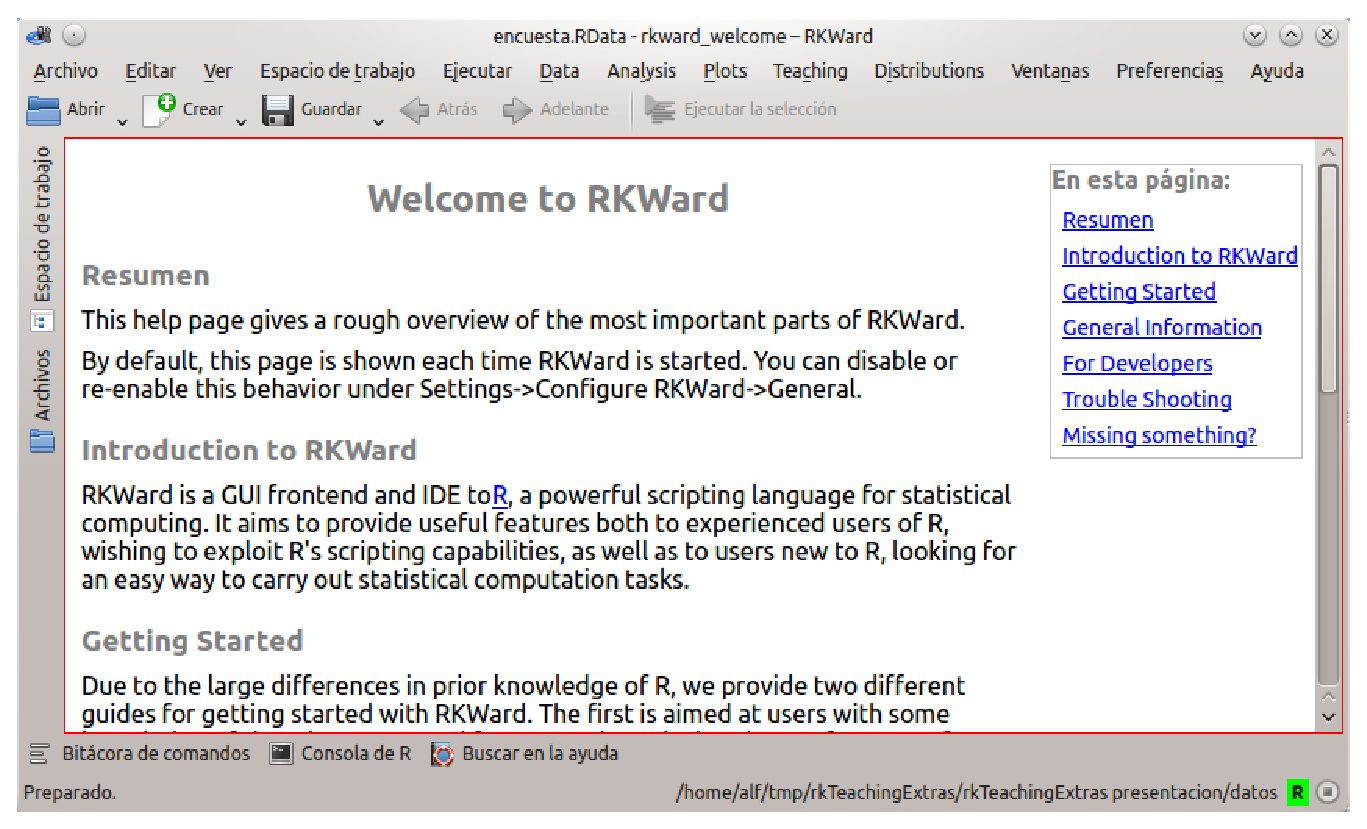
\includegraphics[scale=0.5]{introduccion_r/img/rkward}
  \caption{Interfaz gráfica de usuario de RKWard.}
  \label{g:rkward}
\end{center}
\end{figure}

La interfaz gráfica de usuario RKWard consta de los siguientes elementos:
\begin{itemize}
\item \textbf{Barra de menús}. Contiene distintos menús con operaciones que pueden realizarse con R. 
Si se ha instalado el paquete rkTeaching debe de aparecer el menú Teaching. 
\item \textbf{Barra de botones}. Contiene botones para abrir, crear y guardar conjuntos de datos, espacios de trabajo y guiones de comandos. 
\item \textbf{Ventana principal}. Es la ventana central donde apareceran la ventana de introducción de datos, los resultados de los comandos ejecutados o de las búsquedas realizadas. 
\item \textbf{Espacio de trabajo}. Es una ventana desplegable al hacer clic sobre la solapa situada en el lado izquierdo que contiene todos los elementos del espacio de trabajo de R.
Entre estos elementos aparecen los paquetes cargados, los conjuntos de datos y las variables que contienen los datos de la sesión actual. 
\item \textbf{Bitácora de comandos} Es una solapa desplegable situada en la parte inferior donde aparece un registro de todas las acciones realizadas o comandos ejecutados en la sesión de trabajo actual.
Cada vez que se seleccione un menú que lleve asociado la ejecución de algún comando, dicho comando aparecerá en esta
ventana. Esto permite modificar fácilmente los parámetros del comando y volver a ejecutarlo rápidamente sin necesidad
de volver al menú. 
\item \textbf{Consola de R} Es una solapa desplegable situada también en la parte inferior que da acceso al intérprete de comandos de R.
En esta ventana pueden teclearse y ejecutarse directamente los comandos de R.
\item \textbf{Buscar en la ayuda} Es una solapa desplegable situada en la parte inferior que permite hacer búsquedas sobre comandos de R o de algún paquete.
\item \textbf{Mensajes}. Es la línea de texto que aparece en la parte inferior, donde se muestra información adicional sobre errores, advertencias u
otra información auxiliar al ejecutar un comando, así como la ruta del espacio de trabajo activo.  
\end{itemize}

\section{Tipos de datos y operadores aritméticos y lógicos}
En R existen distintos tipos de datos. Los más básicos son:
\begin{description}
\item[Numeric]: Es cualquier número decimal. Se utiliza el punto como separador de decimales. Por defecto, cualquier
número que se teclee tomará este tipo.
\item[Integer]: Es cualquier número entero. Para convertir un número de tipo Numeric en un entero se utiliza el comando
\lstinline{as.integer()}
\item[Logical]: Puede tomar cualquiera de los dos valores lógicos \lstinline{TRUE} (verdadero) o \lstinline{FALSE}
(falso).
\item[Character]: Es cualquier cadena de caracteres alfanuméricos. Deben introducirse entre comillas. Para convertir
cualquier número en una cadena de caracteres se utiliza el comando \lstinline{as.character()}.
\end{description}

Los valores de estos tipos de datos pueden operarse utilizando distintos operadores o funciones predefinidas para cada
tipo de datos. Los más habituales son:
\begin{description}
\item[Operadores aritméticos]: \lstinline{+} (suma), \lstinline{-} (resta), \lstinline{*} (producto), \lstinline{/}
(cociente), \lstinline{^} (potencia).
\item[Operadores de comparación]: \lstinline{>} (mayor), \lstinline{<} (menor), \lstinline{>=} (mayor o igual),
\lstinline{<=} (menor o igual), \lstinline{==} (igual), \lstinline{!=} (distinto).
\item[Operadores lógicos]:  \lstinline{&} (conjunción y), \lstinline{|} (disyunción o), \lstinline{!} (negación no).
\item[Funciones predefinidas]: \lstinline{sqrt()} (raíz cuadrada), \lstinline{abs()} (valor absoluto),
\lstinline{log()} (logarítmo neperiano), \lstinline{exp()} (exponencial), \lstinline{sin()} (seno), \lstinline{cos()}
(coseno), \lstinline{tan()} (tangente).
\end{description}

Al evaluar las expresiones aritméticas existe un orden de prioridad entre los operadores de manera que primero se
evaluan las funciones predefinidas, luego las potencias, luego los productos y cocientes, luego las sumas y restas,
luego los operadores de comparación, luego las negaciones, luego las conjunciones y finalmente las disyunciones. Para
forzar un orden de evaluación distinto del predefinido se pueden usar paréntesis. Por ejemplo
\begin{lstlisting}
> 2^2+4/2
[1] 6
> (2^2+4)/2
[1] 4
> 2^(2+4/2)
[1] 16
> 2^(2+4)/2
[1] 32
> 2^((2+4)/2)
[1] 8
\end{lstlisting}

También es posible asignar valores a variables mediante el operador de asignación \lstinline{=}. Una vez definidas, las
variables pueden usarse en cualquier expresión aritmética o lógica. Por ejemplo,
\begin{lstlisting}
> x=2
> y=x+2
> y
[1] 4
> y>x
[1] TRUE
> x>=y
[1] FALSE
> x==y-2
[1] TRUE
> x!=0 & !y<x
[1] TRUE
\end{lstlisting}


\section{Introducción y manipulación de datos}
Antes de realizar cualquier análisis de datos hay que introducir los datos que se quieren analizar. 


\subsection{Introducción de datos en línea de comandos}
Existen muchas formas de introducir datos en R pero aquí sólo veremos las más habituales. La forma más rápida de
introducir datos es usar la consola de R para crear un vector de datos mediante el comando \lstinline{c()}. Por ejemplo, para introducir las notas de 5
alumnos se debe teclear en la consola de R
\begin{lstlisting}
> nota = c(5.6,7.2,3.5,8.1,6.4)
\end{lstlisting}
Esto crea el vector \variable{nota} con el que posteriormente se pueden realizar cálculos como por ejemplo la
media
\begin{lstlisting}
> mean(nota)
[1] 6.16
\end{lstlisting}

Otra forma habitual de introducir los datos de una muestra es crear un conjunto de datos mediante el comando
\lstinline{data.frame()}. Por ejemplo, para crear un conjunto de datos a partir de las notas anteriores, hay que teclear
\begin{lstlisting}
> curso = data.frame(nota)
\end{lstlisting}
Esto crea una matriz de datos en la que cada columna se corresponde con una variable y cada fila con un individuo de la
muestra. En el ejemplo la matriz \variable{curso} sólo tendría una columna que se correspondería con las notas y 5
filas, cada una de ellas correspondiente a un alumno de la muestra. Es posible acceder a las variables de un conjunto de
datos con el operador dolar \lstinline{$}. Por ejemplo, para acceder a las notas hay que teclear
\begin{lstlisting}
> curso$nota
[1] 5.6 7.2 3.5 8.1 6.4
\end{lstlisting}
Es fácil añadir nuevas variables a un conjunto de datos, pero siempre deben tener el mismo tamaño muestral. Por ejemplo,
para añadir una nueva variable con el grupo (mañana o tarde) de los alumnos, hay que teclear
\begin{lstlisting}
> curso$grupo = c("m","t","t","m","m")
\end{lstlisting}
Ahora el conjunto de datos \variable{curso} tendría dos columnas, una para la nota y otra para el grupo de los alumnos.
Tecleando el nombre de cualquier objeto, se muestra su información:
\begin{lstlisting}
> curso
   nota   grupo
1   5.6      m
2   7.2      t
3   3.5      t
4   8.1      m
5   6.4      m
\end{lstlisting}

Cuando se introducen datos se puede utilizar el código \lstinline{NA} (not available), para indicar la ausencia del
dato.

Las variables definidas en cada sesión de trabajo quedan almacenas en la memoria interna de R en lo que se conoce como
\emph{espacio de trabajo}.
Es posible obtener un listado de todos los objetos almacenados en el espacio de trabajo mediante los comandos
\lstinline{ls()}.
Si se desea más información, el comando \lstinline{ls.str()} además de mostrar los objetos de la memoria indica sus
tipos y sus valores.
\begin{lstlisting}
> ls()
[1] "curso" "nota"  "x"     "y"    
> ls.str()
curso : 'data.frame':   5 obs. of  2 variables:
 $ nota : num  5.6 7.2 3.5 8.1 6.4
 $ grupo: chr  " m " " t " " t " " m " ...
nota :  num [1:5] 5.6 7.2 3.5 8.1 6.4
x :  num 2
y :  num 4
\end{lstlisting}

Para eliminar un objeto de la memoria se utiliza el comando \lstinline{rm()}.
\begin{lstlisting}
> ls()
[1] "curso" "nota"  "x"     "y"    
> rm(x,y)
> ls()
[1] "curso" "nota"
\end{lstlisting}


\subsection{Introducción de datos en RKWard}
RKWard dispone de una interfaz gráfica para introducir los datos sin necesidad de saberse los comandos anteriores.
Para ello hay que ir al menu \menu{Archivo>Nuevo >Conjunto de datos}. Con esto
aparecerá una ventana donde hay que darle un nombre al conjunto de datos y tras esto aparece la ventana de la
figura~\ref{g:matriz_datos} con una tabla en la que se pueden introducir los datos de la muestra.
Al igual que antes, cada variable debe introducirse en una columna y cada individuo en una fila.

\begin{figure}[htp]
\begin{center}
  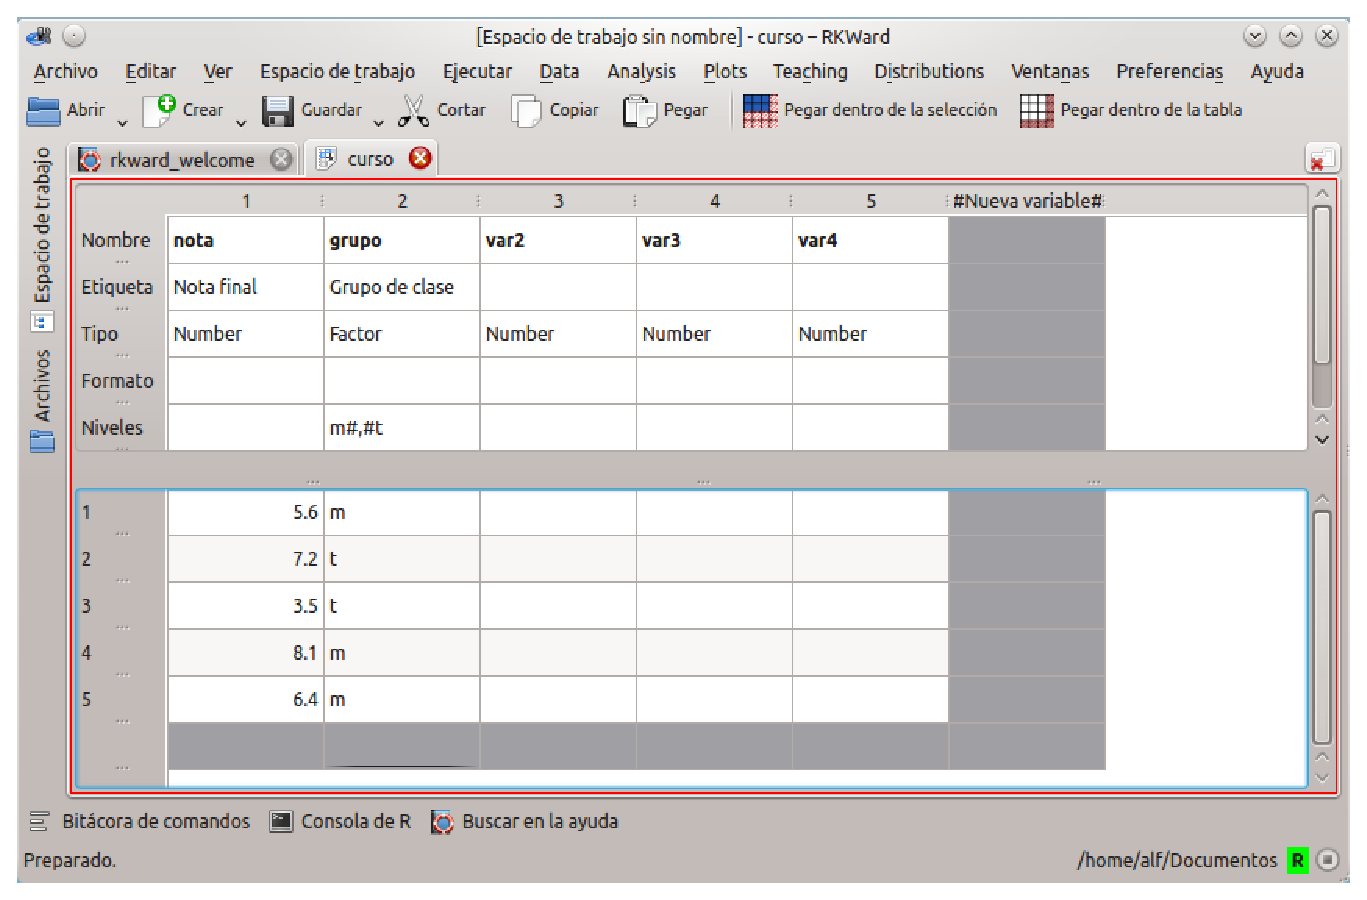
\includegraphics[scale=0.6]{introduccion_r/img/matriz_datos}
  \caption{Ventana de introducción de datos}
  \label{g:matriz_datos}
\end{center}
\end{figure}

Haciendo clic en las casillas de la cabecera cada fila es posible cambiar el nombre de la variable, ponerle una
etiqueta, su tipo, su formato y los niveles en caso de tratarse de un factor o variable categórica.
Los nombres de variables deben comenzar con una letra o un punto y pueden contener cualquier letra, punto, subrayado
(\lstinline{_}) o número.
En particular, no se pueden utilizar espacios en blanco.
Además, R es distingue entre mayúsculas y minúsculas.

Una vez definida la variable, para introducir los datos basta con teclearlos en las casillas que aparecen más abajo en
la misma columna.

R permite definir más de un conjunto de datos en un mismo espacio de trabajo.

Los objetos definidos en el espacio de trabajo pueden verse haciendo clic en la solapa \menu{Espacio de trabajo}.
Para editar una variable o un conjunto de datos basta con hacer doble clic sobre él.
También puede obtenerse un resumen como el que se muestra en la figura~\ref{g:resumen_datos} haciendo clic en el botón
derecho y seleccionando \menu{ver} en el menú contextual que aparece.

\begin{figure}[htp]
\begin{center}
  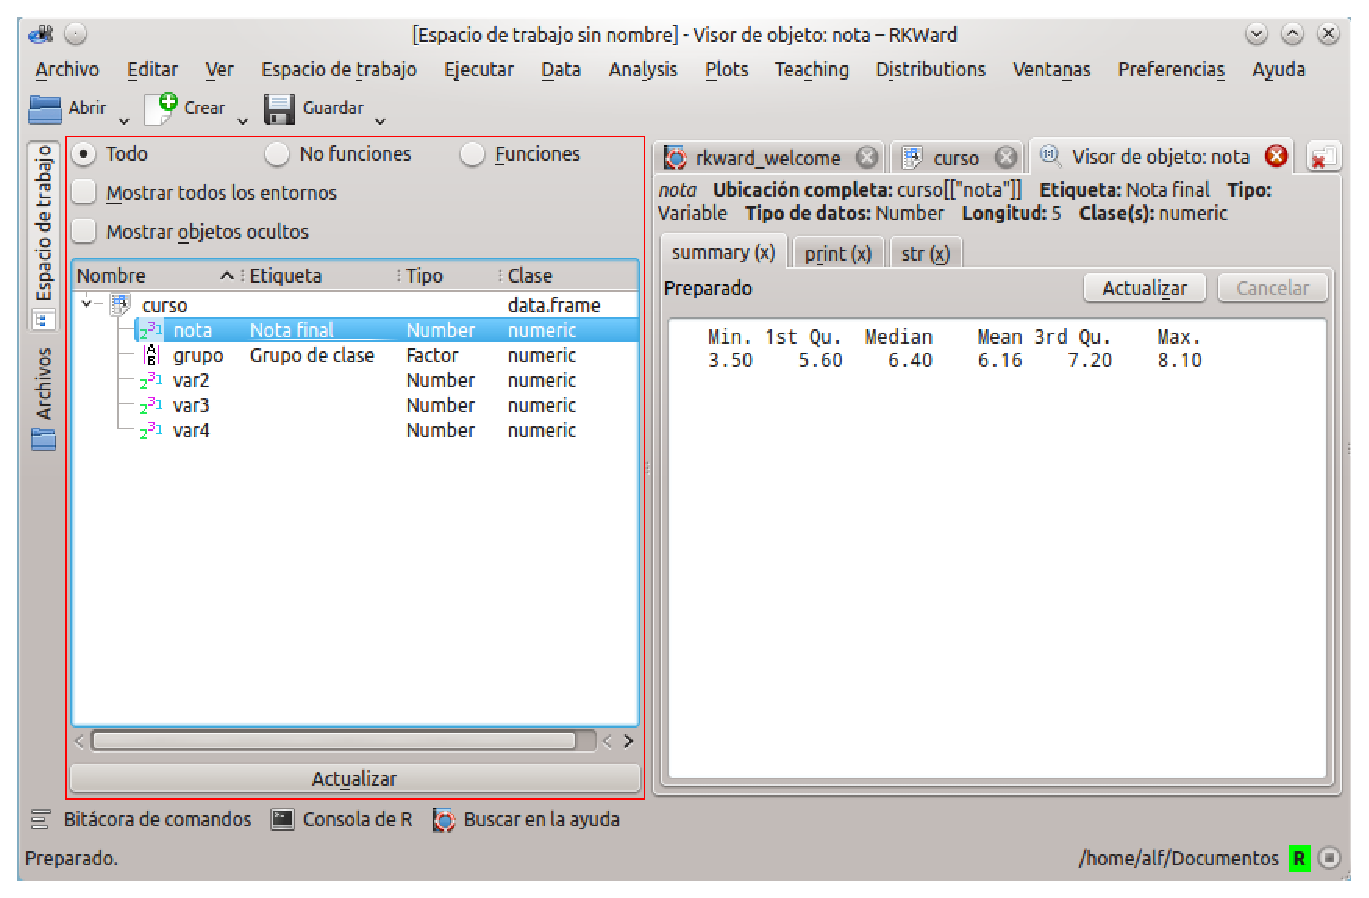
\includegraphics[scale=0.6]{introduccion_r/img/resumen_datos}
  \caption{Ventana de resumen descriptivo de un conjunto de datos}
  \label{g:resumen_datos}
\end{center}
\end{figure}

\subsection{Ponderación de datos}
Cuando una variable o un conjunto de datos tiene unos pocos valores que se repiten mucho, en lugar de teclearlos es más
rápido indicar los valores y ponderarlos por sus frecuencias.
Para ello se utiliza el menú \menu{Teaching>Datos>Ponerar datos}.
Al seleccionarlo aparece una ventana donde hay que seleccionar el conjunto de datos a ponderar, la variable numérica de
dicho conjunto de datos que contiene las frecuencias de ponderación, e indicar un nombre para el nuevo conjunto de datos.
Por ejemplo, si en una clase hay 20 chicas y 30 chicos, se puede crear un conjunto de datos con la variables sexo y
frequencia, tal y como se muestra en la figura~\ref{g:ponderar_variable1}, y después llamar al menú de ponderación con
los datos que aparencen la figura~\ref{g:ponderar_variable2}.

\begin{figure}[htp]
\begin{center}
  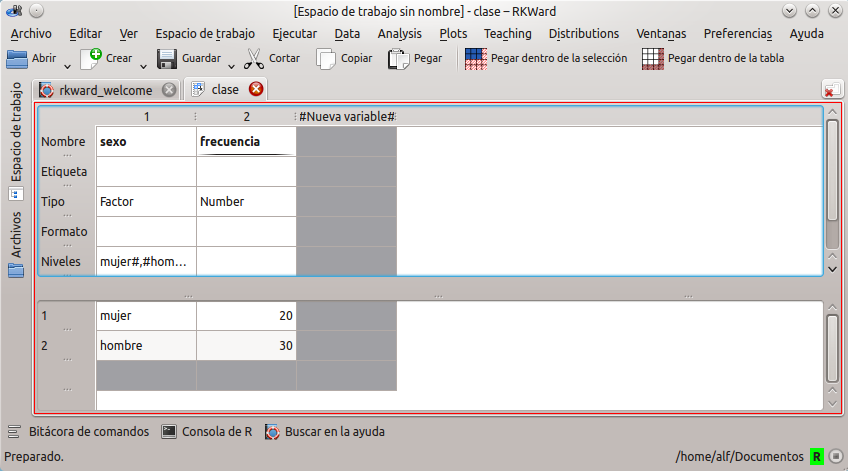
\includegraphics[scale=0.6]{introduccion_r/img/datos_frecuencias}
  \caption{Conjunto de datos preparado para ser ponderado}
  \label{g:ponderar_variable1}
\end{center}
\end{figure}

\begin{figure}[htp]
\begin{center}
  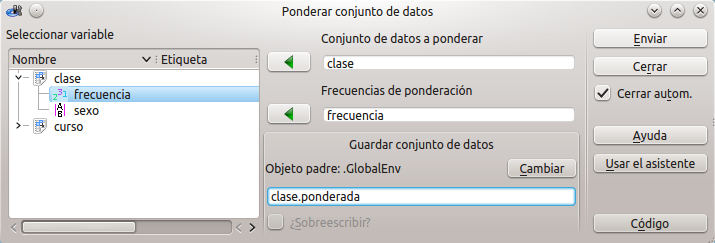
\includegraphics[scale=0.6]{introduccion_r/img/ponderacion}
  \caption{Ventana de ponderación de datos}
  \label{g:ponderar_variable2}
\end{center}
\end{figure}


\subsection{Guardar datos}
Una vez introducidos los datos, conviene guardarlos en un fichero para no tener que volver a introducirlos en futuras
sesiones. Para guardar los conjunto de datos definidos en el espacio de trabajo, se utiliza el menú \menu{Espacio de
trabajo>Guardar espacio de trabajo}.
Con esto aparece una ventana donde hay que darle un nombre al fichero y seleccionar la carpeta donde se guardará.
Los conjuntos de datos se guardan siempre en ficheros de R con extensión \comando{rda} o \comando{rData}.

También es posible guardar los datos en un fichero de texto plano mediante el menú \menu{Archivo>Exportar\flecha
Export tabular data}.
Tras esto aparece una ventana donde hay que seleccionar el conjunto de datos a exportar, darle un nombre al fichero de
texto y seleccionar la carpeta donde se guardará.
Esta ventana contiene también solapas donde se puede indicar entre otras cosas si incluir los nombres de las variables o
no, el separador de decimales o el separador de los datos, que puede ser un espacio, tabuladores, comas u otro caracter.


\subsection{Abrir datos}
Si los datos con los que se pretende trabajar ya están guardados en un fichero de R, entonces tendremos que abrir dicho
fichero. Para ello se utiliza el \menu{Espacio de trabajo>Abrir espacio de trabajo} y en la ventana que aparece
se selecciona el fichero que se desea abrir.
Automáticamente se cargará el conjunto de datos del fichero y pasará a ser el conjunto de datos activo.

También es posible cargar datos de ficheros con otros formatos, como por ejemplo un fichero de texto.
Para ello se utiliza el menú \menu{Archivo>Importar>Importar datos} y en la ventana que aparece se
selecciona el fichero de texto que se desea abrir y en el cuadro desplegable del formato de archivo se debes seleccionar
\opcion{Text}.
Después aparecerá una ventana donde habrá que darle un nombre al conjunto de datos y seleccionar el tipo de separador y
si los nombres de las variables aparecen en la primera línea del fichero.


\subsection{Eliminación de datos}
Para eliminar una variable del conjunto de datos primero hay que editar el conjunto de datos, y después, en la ventana
de edición de datos, hay que hacer clic con el botón derecho del ratón sobre la cabecera de la columna correspondiente
y seleccionar en el menú contextual que aparece \menu{Borrar esta variable}.

Para eliminar individuos del conjunto de datos que hacer clic con el botón derecho del ratón sobre la cabecera de la
fila correspondiente y seleccionar en el menú contextual que aparece \menu{Borrar esta fila}.

En la ventana del espacio de trabajo también es posible borrar cualquier objeto del espacio de trabajo de R haciendo
clic con el botón derecho del ratón sobre él y seleccionando el menú \menu{Eliminar}.


\section{Transformación de datos}
A menudo en los análisis hay que realizar transformaciones en los datos originales.
A continuación se presentan las transformaciones más habituales.


\subsection{Filtrado de datos}
Cuando se desea realizar un análisis con un subconjunto de individuos del conjunto de datos activo que cumplen una
determinada condición es posible filtrar el conjunto de datos para quedarse con esos individuos.
Para ello se utiliza el menú \menu{Teaching>Datos>Filtrar}.
Con esto aparece un cuadro de diálogo en el que hay que seleccionar el conjunto de datos que se desea filtrar, y en el
cuadro de texto \opcion{Condición de selección} indicar la condición lógica que tienen que cumplir los individuos
seleccionados.
También hay que indicar el nombre del nuevo conjunto de datos.
Por ejemplo, para seleccionar los alumnos del grupo de la mañana habría que indicar la condición
\lstinline{grupo==''m''} tal y como se muestra en la figura~\ref{g:filtrar_datos}.

\begin{figure}[htp]
\begin{center}
  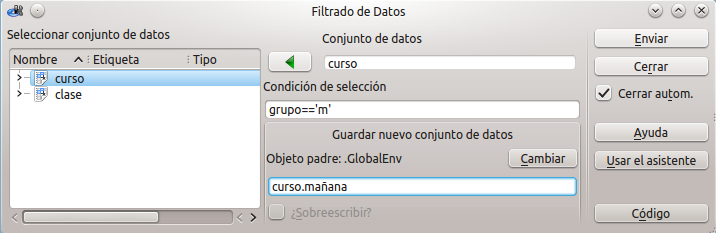
\includegraphics[scale=0.6]{introduccion_r/img/filtrar}
  \caption{Ventana de filtrado de datos.}
  \label{g:filtrar_datos}
\end{center}
\end{figure}


\subsection{Cálculo de variables}
Para calcular una nueva variable a partir de otras ya existentes en el espacio de trabajo de R se utiliza el menú
\menu{Teaching>Datos>Calcular variable}.
Con esto aparece un cuadro de diálogo en el que hay que introducir la expresión a partir de la que se calculará la nueva
variable en el cuadro de texto \opcion{Expresión de cálculo}, e indicar el nombre de la nueva variable.
La expresión de cálculo puede ser cualquier expresión aritmética o lógica de R, en las que pueden utilizarse cualquiera
de las variables del espacio de trabajo de R. Por ejemplo, para eliminar los decimales de la variable \variable{nota}
podría crearse una nueva variable \variable{puntuacion} multiplicando por 10 las notas, tal y como se muestra en la
figura~\ref{g:calcular_variable}.

\begin{figure}[htp]
\begin{center}
  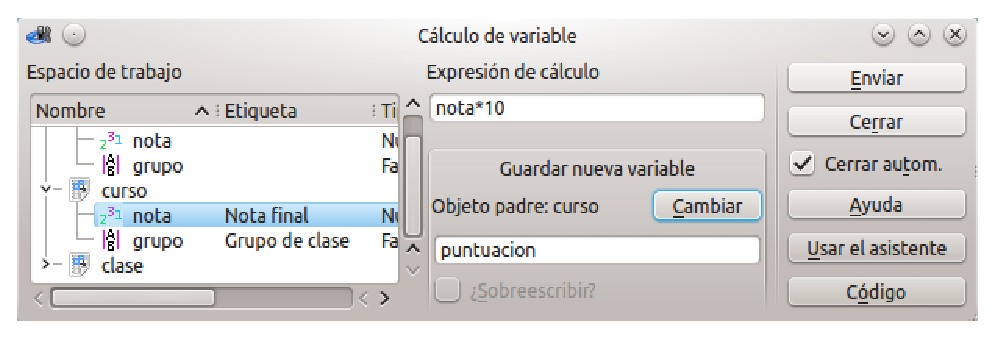
\includegraphics[scale=0.6]{introduccion_r/img/calcular}
  \caption{Ventana de cálculo de nuevas variables.}
  \label{g:calcular_variable}
\end{center}
\end{figure}


\subsection{Recodificación de variables}
Otra transformación habitual es la recodificación de variables que permite transformar los valores de una variable de
acuerdo a un conjunto de reglas de reescritura. Normalmente se utiliza para convertir una variable numérica en una
variable categórica que pueda usarse como un factor. 

Para recodificar una variable se utiliza el menú \menu{Teaching>Datos>Recodificar variable}.
Con esto aparece una ventana en la que hay que seleccionar la variable que se desea recodificar, indicar el nombre de la
nueva variable recodificada e introducir las reglas de recodificación en el cuadro de texto \opcion{Reglas de
recodificación}.
Las reglas de recodificación siempre siguen la sintaxis \lstinline{valor o rango de valores = nuevo valor} y pueden
introducirse tantas reglas como se desee, cada una en una línea.
Al lado izquierdo de la igualdad puede introducirse un único valor, varios valores separados por comas, o un rango de
valores indicando el límite inferior y el límite superior del intervalo separados por el operador \lstinline{:}.
A la hora de definir el límite inferior puede utilizarse la palabra clave \lstinline{lo} para referirse al menor de los
valores de la muestra y \lstinline{hi} para referirse al mayor de los valores.
Por ejemplo, para recodificar la variable \variable{nota} en categorías correspondientes a las calificaciones ([0-5)
Suspenso, [5,7) Aprobado, [7,9) Notable y [9,10] Sobresaliente), habría que introducir las reglas que se muestran en la
figura~\ref{g:recodificar_variable}. Después, en la ventana de introducción de datos, se pueden renombrar los niveles
del factor introduciendo el valor suspenso para la categoría 1, aprobado para la categoría 2, notable para la categoría
3 y sobresaliente para la categoría 4. 

\begin{figure}[htp]
\begin{center}
  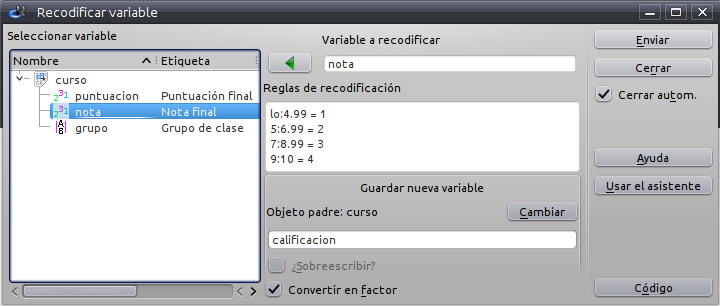
\includegraphics[scale=0.6]{introduccion_r/img/recodificar}
  \caption{Ventana de recodificación de variables}
  \label{g:recodificar_variable}
\end{center}
\end{figure} 


\section{Manipulación de ficheros de resultados}

\subsection{Guardar los resultados}
Cada vez que se ejecuta un comando de R, bien en la consola de comandos o a través de un menú, el comando ejecutado y su
salida quedan registrados en la bitácora de comandos. Sin embargo, esta salida es en texto plano sin formato por lo que
muchos de los procedimientos recogidos en los menús producen además una salida mucho más comprensible en formato HTML en
la ventana de resultados.

Para guardar el contenido de la ventana de resultados en un fichero se utiliza el menú \menu{Archivo>Exportar
página como HTML}.
Con esto aparece un cuadro de diálogo en el que hay que indicar el nombre del fichero y la carpeta donde se desea
guardar. El fichero resultante está en formato HTML por lo que se podrá visualizar con cualquier navegador web.

\subsection{Limpiar la ventana de resultados}
La vetana de resultados va acumulando todas las salidas de los análisis realizados en cada sesión de trabajo. 
Para no mezclar los resultados de estudios distintos, conviene limpiar la ventana de resultados cada vez que se empiece un estudio nuevo.
Para ello hay que seleccionar el menú \menu{Edición>Limpiar salida}.
 

\section{Manipulación de guiones de comandos}

\subsection{Creación de un guión de comandos}
RKWard también incorpora un entorno de desarrollo para programadores de R que permite crear guiones de comandos que
pueden ejecutarse todos seguidos.
Esta opción es muy interesante para repetir análisis o automatizar tareas repetitivas.
Para crear un guión de comandos hay que seleccionar el menú \menu{Archivo>Nuevo>Archivo de guiones}.
Con esto aparecerá una venta como la que aparece en la figura~\ref{g:guiones_comandos} donde se podrán teclecar los
comandos de R para después ejecutarlos uno a uno o en bloque.

\begin{figure}[htp]
\begin{center}
  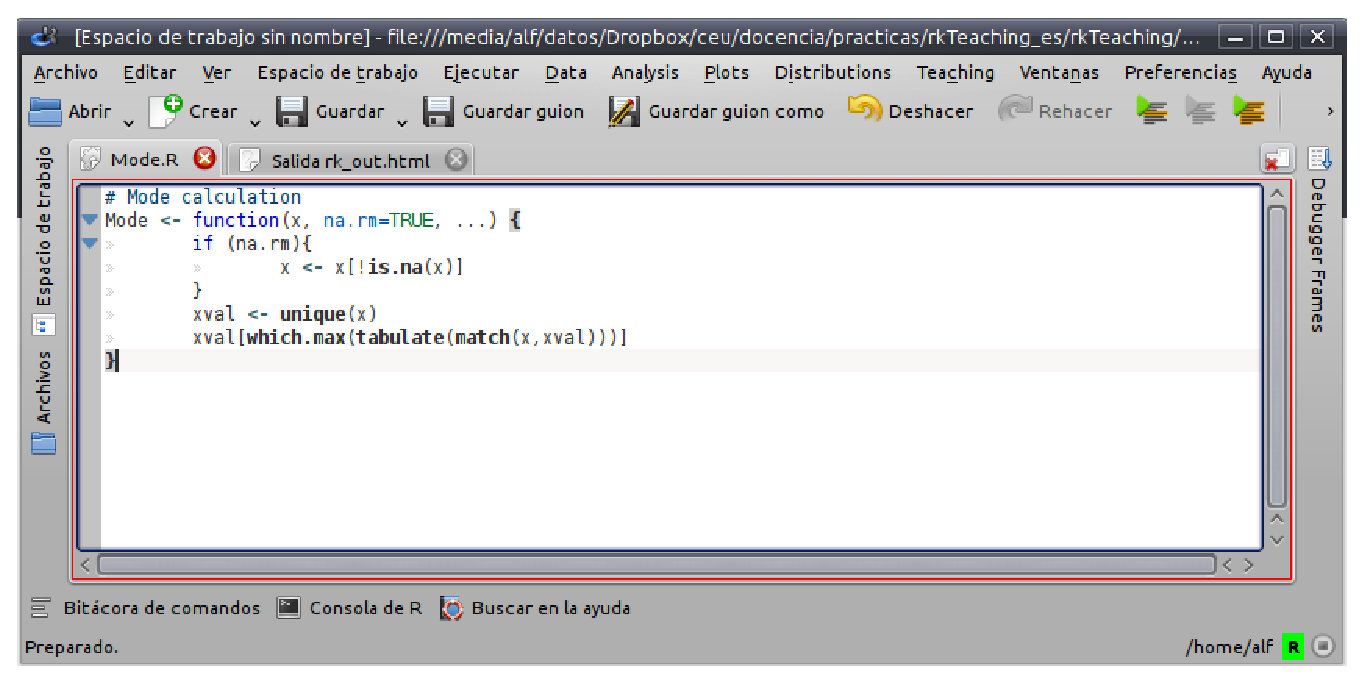
\includegraphics[scale=0.6]{introduccion_r/img/guiones_comandos}
  \caption{Ventana de edición de guiones de comandos}
  \label{g:guiones_comandos}
\end{center}
\end{figure}


\subsection{Guardar un guión de comandos}
Los guiones de comandos también pueden guardarse en un fichero de texto plano mediante el menú
\menu{Archivo>Guardar guión} e indicando el nombre del fichero y la carpeta donde se guardará en el
cuadro de diálo que aparece.


\subsection{Abrir un guión de comandos}
Para abrir un fichero con un guión de comandos se utiliza el menú \menu{Archivo>Abrir archivo de guiones de R} y
después seleccionar el fichero que se desea abrir en el cuadro de diálogo que aparece. 


\section{Ayuda}
Otra de las ventajas de R es que tiene un sistema de ayuda muy documentado. Es posible conseguir ayuda sobre cualquier
función, prodecimiento o paquete simplemente tecleando el comando \lstinline{help()}. Por ejemplo, para obtener ayuda
sobre el comando \lstinline{mean} se teclearía
\begin{lstlisting}
> help("mean")
\end{lstlisting}
y con esto aparecerá una ventana de ayuda donde se describe la función y también aparecen ejemplos que ilustran su uso. 
Si no se conoce exactamente el nombre de la función o comando, se puede hacer una búsqueda aproximada con el comando
\lstinline{help.search()}. Por emplo, si no se recuerda el nombre de la función logarítmica, se podría
teclear
\begin{lstlisting}
> help("logarithm")
\end{lstlisting}
y con esto aparecerá una ventana con todos los ficheros de ayuda que contienen la palabra logarithm.

Finalmente, también es posible invocar la ayuda general de R en RKWard con el menú \menu{Ayuda>Ayuda de R} con lo
que aparecerá una página web desde donde podremos navegar a la información deseada. También es posible buscar ayuda
sobre un comando concreto en el menú \menu{Ayuda>Buscar en la ayuda de R}.

Para más información sobre R se recomienda visitar la página \url{http://www.r-project.org/}, y para más información
sobre RKWard se recomienda visitar la página \url{http://rkward.sourceforge.net/}. 

\clearpage
\newpage

\section{Ejercicios resueltos}
\begin{enumerate}[leftmargin=*]
\item Crear un conjunto de datos con los datos de la siguiente muestra y guardarlo con el nombre
\comando{colesterol.rda}
\begin{center}
\begin{tabular}{|l|c|r|r|r|}
\hline
\multicolumn{1}{|c|}{Nombre} & \multicolumn{1}{c|}{Sexo} & \multicolumn{1}{c|}{Peso} & \multicolumn{1}{c|}{Altura} & \multicolumn{1}{c|}{Colesterol}\\
\hline
José Luis Martínez Izquierdo  & H &  85 & 179 & 182\\
Rosa Díaz Díaz & M & 65 & 173 & 232\\
Javier García Sánchez  & H & 71 & 181 & 191\\
Carmen López Pinzón & M &  65 & 170 & 200\\
Marisa López Collado & M &  51 & 158 & 148\\
Antonio Ruiz Cruz & H & 66 & 174 & 249\\
\hline
\end{tabular}
\end{center}

\begin{indicacion}{Para crear el conjunto de datos:
\begin{enumerate}
\item Seleccionar el menú \menu{Archivo>Nuevo>Conjunto de datos}.
\item En el cuadro de diálogo que aparece introducir el nombre del conjunto de datos \variable{colesterol} y hacer clic en el botón \boton{Aceptar}.
\item En la ventana del editor de datos hay que definir una variable en cada columna introduciendo su nombre y tipo en las casillas de la cabecera de cada columna.
\item Una vez definidas las variables hay que introducir los datos de cada variable en la columna correspondiente. 
\end{enumerate}
Para guardar los datos:
\begin{enumerate}
\item Selecionar el menú \menu{Espacio de trabajo>Guardar espacio de trabajo}.
\item En el cuadro de diálogo que aparece hay que darle un nombre al fichero, seleccionar la carpeta donde guardarlo y hacer clic en el
botón \boton{Aceptar}.
\end{enumerate}
}
\end{indicacion}

\item Abrir el fichero creado en el ejercicio anterior y realizar las siguientes operaciones:

\begin{enumerate}
\item Insertar una nueva variable \variable{Edad} con las edades de todos los individuos de la muestra.
\begin{center}
\begin{tabular}{|l|r|}
\hline
\multicolumn{1}{|c|}{Nombre} & \multicolumn{1}{c|}{Edad} \\
\hline
José Luis Martínez Izquierdo & 18 \\
Rosa Díaz Díaz & 32 \\
Javier García Sánchez & 24 \\
Carmen López Pinzón & 35 \\
Marisa López Collado & 46 \\
Antonio Ruiz Cruz & 68 \\
\hline
\end{tabular}
\end{center}

\begin{indicacion}{ Para abrir el conjunto de datos del ejercicio anterior:
\begin{enumerate}
\item Seleccionar el menú \menu{Espacio de trabajo>Abrir espacio de trabajo}.
\item En el cuadro de diálogo que aparece seleccionar la carpeta donde se encuentra el fichero con los datos del ejercicio anterior,
seleccionar el fichero y hacer clic en el botón \boton{Aceptar}.
\end{enumerate}
Para insertar la variable \variable{Edad}:
\begin{enumerate}
\item Hacer clic en la solapa \boton{Espacio de trabajo}.
\item En la ventana del espacio de trabajo doble clic sobre el conjunto de datos \variable{colesterol}.
\item En la ventana del editor de datos introducir el nombre de la variable \variable{edad} y su tipo en las casillas de la cabecera de una nueva columna vacía, e introducir los datos de las edades en las celdas de maś abajo. 
\end{enumerate}
}
\end{indicacion}

\item Insertar un nuevo individuo con siguientes datos
\begin{quote}
Nombre: Cristóbal Campos Ruiz.\\
Edad: 44 años.\\
Sexo: Hombre.\\
Peso: 70 Kg.\\
Altura: 178 cm.\\
Colesterol: 220 mg/dl.
\end{quote}

\begin{indicacion}{
\begin{enumerate}
\item En la ventana del editor de datos introducir los datos de del nuevo individuo en la primera fila vacía.
\end{enumerate}
}
\end{indicacion}

\item Crear una nueva variable donde se calcule el índice de masa corporal de cada paciente mediante la formula:
\[
\text{imc} = \frac{\text{Peso (en Kg)}}{\text{Altura (en mt)}^2}
\]

\begin{indicacion}{
\begin{enumerate}
\item Seleccionar el menú \menu{Teaching>Datos>Calcular variable}.
\item En el cuadro de diálogo que aparece introducir la fórmula para calcular el índice de masa
corporal en el campo \campo{Expresión de cálculo}.
\item En el cuadro \campo{Guardar nueva variable} hacer clic sobre el botón \boton{Cambiar}.
\item En el cuadro de diálogo que aparece seleccionar como objeto padre la el conjunto de datos \variable{colesterol} y hacer clic sobre el botón \boton{Aceptar}.
\item Introducir el nombre de la nueva variable \variable{imc} y hacer clic sobre el botón \boton{Aceptar}.
\end{enumerate} 
}
\end{indicacion}

\item Recodificar el índice de masa corporal en una nueva variable de acuerdo a las siguientes categorías:
\begin{center}
\begin{tabular}{ll}
Menor de $18.5$ & Bajo peso\\
De $18.5$ a $24.5$ & Saludable\\
De $24.5$ a $30$ & Sobrepeso\\
Mayor de $30$  & Obeso
\end{tabular}
\end{center}

\begin{indicacion}{
\begin{enumerate}
\item Selecionar el menú \menu{Teaching>Datos>Recodificar variable}.
\item En el cuadro de diálogo que aparece seleccionar como variable a recodificar la variable \variable{imc}.
\item Introducir las reglas de recodificación en el campo \campo{Reglas de recodificación}:
\begin{quote}
\lstinline{lo:18.5 = 1}\\
\lstinline{18.5:24.5 = 2}\\
\lstinline{24.5:30 = 3}\\
\lstinline{30:hi = 4}
\end{quote}
\item En el cuadro \campo{Guardar nueva variable} hacer clic sobre el botón \boton{Cambiar}.
\item En el cuadro de diálogo que aparece seleccionar como objeto padre la el conjunto de datos \variable{colesterol} y hacer clic sobre el botón \boton{Aceptar}.
\item Introducir el nombre de la nueva variable \variable{obesidad} y hacer clic sobre el botón \boton{Aceptar}.
\item En la ventada de edición de datos introducir los niveles del factor, asignando Bajo peso a la categoría 1,
Saludable a la categoría 2, Sobrepeso a la categoría 3 y Obeso a la categoría 4. 
\end{enumerate}
}
\end{indicacion}


\item Filtrar el conjunto de datos para obtener un nuevo conjunto de datos con los datos de los hombres
\begin{indicacion}{
\begin{enumerate}
\item Selecionar el menú \menu{Teaching>Datos>Filtrar}.
\item En el cuadro de diálogo que aparece seleccionar como conjunto de datos \variable{colesterol}.
\item En el campo \campo{Condición de selección} introducir la condición \lstinline{sexo=="H"}. 
\item Introducir el nombre del  nuevo conjunto de datos \variable{colesterol.hombres} y hacer clic sobre el botón \boton{Aceptar}.
\end{enumerate}
}
\end{indicacion}
%\item Importar el conjunto de datos del fichero de texto \comando{Nations.txt} que se encuentra en el subdirectorio \comando{etc} del
% paquete \comando{Rcmdr} y visualizar el conjunto de datos.

%\item Filtrar el conjunto de datos para quedarse únicamente con los países de Europa.

\end{enumerate}
\end{enumerate}

\section{Ejercicios propuestos}
\begin{enumerate}[leftmargin=*]
\item  El conjunto de datos \variable{neonatos} del paquete \variable{rk.Teaching}, contiene información sobre una
muestra de 320 recién nacidos en un hospital durante un año que cumplieron el tiempo normal de gestación. 
Se pide:
\begin{enumerate}
\item Cargar el conjunto de datos.
\begin{indicacion}{
\begin{enumerate}
\item Hacer clic en la solapa \campo{Espacio de trabajo} para desplegarla y ver los paquetes del espacio de trabajo. 
\item Hacer doble clic sobre el paquete \variable{rk.Teaching} para ver todos los conjuntos de datos que contiene. 
\item Hacer clic con el botón derecho sobre el conjunto de datos \variable{nenonatos} y en el menú contextual que
aparece selecconar \menu{Copiar a .GlobalEnv} para hacer una copia del conjunto de datos en nuestro entorno de trabajo. 
\end{enumerate}
}
\end{indicacion}

\item Calcular la variable \variable{apgar.medio} como la media de las variables \variable{apgar1} y \variable{apgar5}.
\item Recodificar la varible \variable{peso} en el factor \variable{categoria.peso} con dos categorias que se
correspondan con los pesos menores y mayores de $2.5$ Kg.
\item Recodificar la variable \variable{apgar1} en el factor \variable{estado.apgar1} con tres categorías: deprimido
(Apgar$\leq 3$), moderadamente deprimido ($3<$Apgar$\leq 6$) y normal (Apgar$>6$).
\item Filtrar el conjunto de datos para quedarse con los hijos de las madres no fumadoras con una puntuación Apgar al
minuto de nacer menor o igual que 3. ¿Cuántos niños hay?
\end{enumerate}
\end{enumerate}